%!TEX root = ../thesis.tex
%*******************************************************************************
%****************************** Second Chapter *********************************
%*******************************************************************************

\chapter{Fermion-to-Qubit Mappings}

\ifpdf
    \graphicspath{{Chapter2/Figs/Raster/}{Chapter2/Figs/PDF/}{Chapter2/Figs/}{Chapter2/hybrid_mapping/}}
\else
    \graphicspath{{Chapter2/Figs/Vector/}{Chapter2/Figs/}{Chapter2/hybrid_mapping/}}
\fi


\section[Hybrid Mappings]{Hybrid Fermion-to-Qubit Mappings}
\begin{table}
\centering
\small
    \begin{tabular}{k{6em} k{4.3em} k{4.5em} k{4.6em} k{5em} k{4.6em}}
        \hline \hline
         & Qubit to fermion ratio  &Max Pauli string & Avg. Pauli string & Avg. Range & Max Range\\ \hline \rowcolor{Gray}
        
        \begin{mytabular}[1]{c}Jordan-\\Wigner~\cite{jordan1993paulische}\end{mytabular}&1&$2N$&$\frac{N}{2} +\frac{3}{2}$&$\frac{N}{2} +\frac{3}{2}$&N+1 \\
        \begin{mytabular}[1]{c}Bravyi-\\Kitaev~\cite{bravyi2002fermionic}\end{mytabular}  &
        1&$\mathcal{BK}_{N^2}$&$\overline{\mathcal{BK}}_{N^2}$&$O(\frac{N}{2})$*& O(N)\\\rowcolor{Gray}
        \begin{mytabular}[1]{c}$n\times n$\\{\bf  Hybrid}\end{mytabular}&$1$&\begin{tabular}{c}$\frac{2N}{n} +$\\ $2\mathcal{BK}_{n^2}$\end{tabular}&\begin{tabular}{c}$\frac{N}{2n^2} +$\\ $\frac{n+1}{n}\overline{\mathcal{BK}}_{n^2}$\end{tabular}&$O(\frac{N}{2n}+\frac{n}{2})$&$O(\frac{N}{n}+n)$ \\
        \begin{mytabular}[1]{c}Derby-\\Klassen~\cite{derby2021compact} \end{mytabular}&1.5&$3$&$3$&$3$& 3\\\rowcolor{Gray}
        \begin{mytabular}[1]{c}Super-\\compact~\cite{chen2022equivalence} \end{mytabular}&1.25&$6$&$O(1)$&$O(1)$&O(1) \\
        AQM~\cite{Verstraete_2005,steudtner2019quantum}&$2-\frac{1}{N}$&$6$&$O(1)$&$O(1)$&O(1) \\\rowcolor{Gray}
        \begin{mytabular}[1]{c}$n\times n$\\{\bf  Hybrid\+}\end{mytabular}&$1+\frac{1}{n^2}$&\begin{mytabular}[1.2]{c}$3 +$ \\ $2\mathcal{BK}_{n^2}$\end{mytabular}&\begin{tabular}{c}$\frac{2}{n} +\frac{1}{n^2}+$\\ $\frac{n+1}{n}\overline{\mathcal{BK}}_{n^2}$\end{tabular}&$O(\frac{n}{2})$*& $O(n)$\\
        Low-ratio mapping~\cite{chen2022equivalence,steudtner2019quantum}&$1+\frac{1}{k}$&$O(k)$&$O(k)$&$O(k)$& $O(k)$\\ \hline
    \end{tabular}
    \caption{\label{tab:performance} { Comparison of the performance (on an $N \times N$ square-lattice fermionic interaction graph) of select families of fermion-to-qubit mappings including state-of-the-art alongside our novel mapping $n\times n$ Hybrid and Hybrid\+ mappings for $n \ll N$.  $\mathcal{BK}_m$ and $\overline{\mathcal{BK}}_m$ represent the $O(\log m)$ maximum and average Pauli-weight of fermionic operators under the Bravyi-Kitaev mapping on $m$ fermionic modes. For each hybrid mapping, $n$ is fixed. For $n=1$ the Hybrid mapping is equivalent to the Jordan-Wigner mapping, and the Hybrid\+ mapping is equivalent to AQM. For $n=N$ both are equivalent to the Bravyi-Kitaev mapping. Intermediate values of $n$ combine the strengths of these mappings to give improved performance. The optimal choice of $n$ is dependant upon $N$ and must be found numerically (Figures~\ref{fig:vary_cell_sizes_32},\ref{fig:vary_cell_sizes_64}). For $N=64$, the optimal choice is $n=8$. The $8 \times 8$ Hybrid mapping gives 98\% shorter Pauli-strings than the Jordan-Wigner mapping, and the $8 \times 8$ Hybrid\+ mapping only requires 1.016 qubits per fermion. This is 94\% fewer ancillae than the super-compact mapping (which requires the fewest ancillae of all known local mappings). *These values are estimated using numerical evaluation.} } 
\end{table}

We present two novel mapping algorithms: Hybrid mapping (Section~\ref{section:Hybridmapping}) and Hybrid\+ mapping (Section~\ref{section:auxHybridmapping}). The Hybrid mapping combines the low connectivity constraints of the Jordan-Wigner mapping with the increased locality of the Bravyi-Kitaev mapping. The Hybrid\+ mapping builds on the strengths of the Hybrid mapping and expands the mapping to include aspects of AQM \cite{Verstraete_2005, steudtner2019quantum} to increase the locality using ancilla qubits.
In this section we outline their construction in detail, and then in Section~\ref{section:algorithmanalysis} we will analyse their performance. 
Both these mappings have been designed for a square-lattice fermionic interaction graph. For the sake of clarity, they are both described with $n \times n$ cells, however, it is trivial to extend them to rectangular $l \times h$ cells. It is also possible to perform these mappings with irregular varying cell sizes. We note that it is possible to extend this mapping to any connectivity or fermionic interaction graph, one must simply make an appropriate choice of cells to split the graph into and then pick an order in which to connect them via Jordan-Wigner.
\subsection{Hybrid mapping algorithm}
\label{section:Hybridmapping}
\noindent
\textbf{Input:} \textit{$N\times N$ Fermion Square-Lattice Interaction Graph, Cell Shape $n \times n$}, $1\le n\le N$ and $n$ is a factor of $N$\\
\textbf{Output:} \textit{Pauli-strings corresponding to interaction edges, Enumerated square-lattice of qubits}\\
\textbf{Summary:} This mapping effectively splits up the square lattice into a series of Fenwick trees (Bravyi-Kitaev maps) and connects them via a Jordan-Wigner mapping on the roots, as demonstrated in \Cref{fig:fenwick_tree_cells,fig:fenwick_tree_cells_example_1,fig:fenwick_tree_cells_example_2,fig:fenwick_tree_cells_example_3,fig:fenwick_tree_cells_example_4}. These diagrams show how creation and annihilation operators are mapped to Jordan-Wigner like $ZZ\ldots ZX$ strings on the roots of previous trees and Bravyi-Kitaev like strings within the current tree.\\
\textbf{Algorithm:}
\begin{enumerate}
    \item Divide the square lattice of fermions into cells of size $n \times n$
    \item Assign a \textit{cell number} $(c_i)$ to each of these cells in a Z pattern starting with the top-left most cell (illustrated by Figure~\ref{ZPattern} in the Appendix). 
    This enumeration reflects the Jordan-Wigner-esque properties of the mapping.
    \item Within these cells assign each fermion a \textit{mode number} $(f_i)$ from $1$ to $n\times n$ in a Z pattern starting with the top-left most fermion. We can now refer to the $i$-th fermion in the graph via the coordinate $(c_i, f_i)$.
    \item Repeat this procedure on a square qubit lattice of the same size so for every fermion there is an equivalent qubit labeled with the same coordinate
    \item For each interaction edge in your fermion interaction graph between $(c_1, f_1)$ and $(c_2, f_2)$ generate the Pauli-string representation:
    \begin{enumerate}
        \item Generate the update $U_i$, flip $F_i$, and parity $P_i$ sets for $f_1$ and $f_2$ independently in a Fenwick tree of size $n \times n$\\
        \textsc{$U_i = (c_i, $ \hyperref[GenerateUpdateSet]{GenerateUpdateSet}($f_i, n\times n$))}\\
        \textsc{$F_i = (c_i, $ \hyperref[GenerateFlipSet]{GenerateFlipSet}($f_i$))}\\
        \textsc{$P_i = (c_i, $ \hyperref[GenerateParitySet]{GenerateParitySet}($f_i$))}
        \item Add the roots of every cell lower in the Z pattern than $c_1$ and $c_2$ to their respective parity sets. \\
        \textsc{For all $c_j < c_1$ add $(c_j, n \times n)$ to $P_1$}\\
        \textsc{For all $c_j < c_2$ add $(c_j, n \times n)$ to $P_2$}
        \item Pauli-string representation is given by:\\
            \begin{dmath*}[style={\footnotesize}]
                    a_1a^{\dagger}_2  \rightarrow X_{U_1}  \sigma^-_1  Z_{P_1/F_1}  X_{U_2}  \sigma^+_2Z_{P_2/F_2}
                    = \frac{1}{4}\left( \bigotimes_{j \in U_1} X_j \otimes X_{(c_1, f_1)} \otimes \bigotimes_{j \in P_1} Z_j +\i \bigotimes_{j \in U_1} X_j \otimes Y_{(c_1, f_1)}\otimes \bigotimes_{j \in P_1/F_1} Z_j \right)\\ \left( \bigotimes_{j \in U_2} X_j \otimes X_{(c_2, f_2)} \otimes \bigotimes_{j \in P_2} Z_j - i \bigotimes_{j \in U_2} X_j \otimes Y_{(c_2, f_2)}\otimes \bigotimes_{j \in P_2/F_2} Z_j \right) = \frac{1}{4}\bigotimes_{j \in (U_1 \oplus U_2)} X_j \bigotimes_{j \in (P_1/F_1 \oplus P_2/F_2)} Z_j \otimes \left( X_{(c_1, f_1)} \otimes \bigotimes_{j \in F_1} Z_j + i Y_{(c_1, f_1)} \right) \left( X_{(c_2, f_2)} \otimes \bigotimes_{j \in F_2} Z_j - i  Y_{(c_2, f_2)} \right) 
            \end{dmath*}    
    \end{enumerate}
\end{enumerate}
\begin{figure}[hbtp] 
        \centerline{
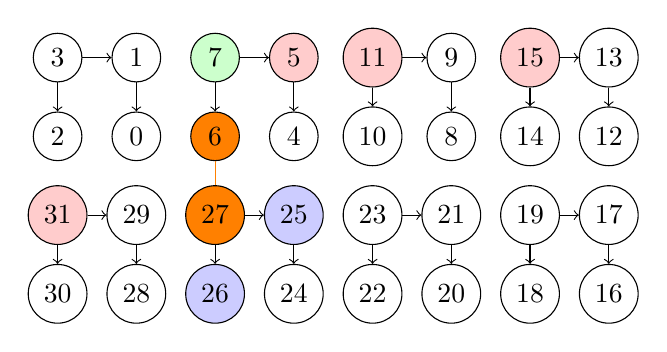
\begin{tikzpicture}[nodes={draw, circle}, ->]
        \node (3) at (0,1) {3};
        \node (1) at (1,1) {1};
        \node (0) at (1,0) {0};
        \node (2) at (0,0) {2};
        \draw [->] (3) -- (1);
        \draw [->] (3) -- (2);
        \draw [->] (1) -- (0);
        \node[fill = green!20] (7) at (2,1) {7};
        \node[fill = red!20]  (5) at (3,1) {5};
        \node (4) at (3,0) {4};
        \node[fill = orange] (6) at (2,0) {6};
        \draw [->] (7) -- (5);
        \draw [->] (7) -- (6);
        \draw [->] (5) -- (4);
        \node[fill = red!20] (11) at (0,-1) {31};
        \node (9) at (1,-1) {29};
        \node (8) at (1,-2) {28};
        \node (10) at (0,-2) {30};
        \draw [->] (11) -- (9);
        \draw [->] (11) -- (10);
        \draw [->] (9) -- (8);
        \node[fill = orange] (27) at (2,-1) {27};
        \node[fill = blue!20]  (13) at (3,-1) {25};
        \node (12) at (3,-2) {24};
        \node[fill = blue!20]  (14) at (2,-2) {26};
        \draw [->] (27) -- (13);
        \draw [->] (27) -- (14);
        \draw [->] (13) -- (12);
        
        \node[fill = red!20] (11) at (4,1) {11};
        \node (9) at (5,1) {9};
        \node (8) at (5,0) {8};
        \node (10) at (4,0) {10};
        \draw [->] (11) -- (9);
        \draw [->] (11) -- (10);
        \draw [->] (9) -- (8);
        \node[fill = red!20] (15) at (6,1) {15};
        \node (13) at (7,1) {13};
        \node (12) at (7,0) {12};
        \node (14) at (6,0) {14};
        \draw [->] (15) -- (13);
        \draw [->] (15) -- (14);
        \draw [->] (13) -- (12);
        \node  (23) at (4,-1) {23};
        \node (9) at (5,-1) {21};
        \node (8) at (5,-2) {20};
        \node (26) at (4,-2) {22};
        \draw [->] (23) -- (9);
        \draw [->] (23) -- (26);
        \draw [->] (9) -- (8);
        \node  (19) at (6,-1) {19};
        \node (13) at (7,-1) {17};
        \node (12) at (7,-2) {16};
        \node (14) at (6,-2) {18};
        \draw [->] (19) -- (13);
        \draw [->] (19) -- (14);
        \draw [->] (13) -- (12);
        \draw [-, orange] (6) -- (27);
\end{tikzpicture}}
\caption{\label{fig:fenwick_tree_cells} Hybrid mapping with $2\times 2$ cells showing the different sets of qubits involved in a fermionic operation between mode 6 and 27. Orange = targets, Blue = Flip set, Red = Parity set, Green = Update set}
\end{figure}
\begin{figure}[hbtp] 
        \centerline{
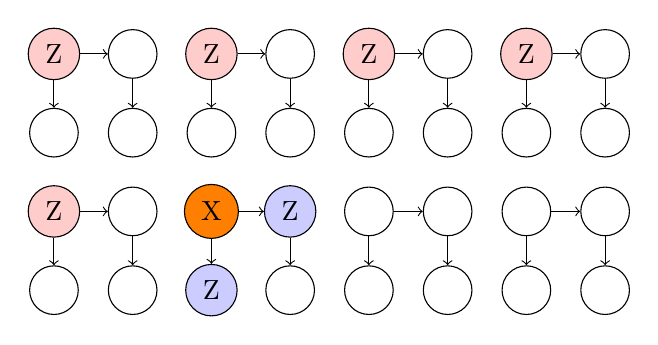
\begin{tikzpicture}[nodes={draw, circle}, ->]
        \node[fill = red!20] (3) at (0,1) {Z};
        \node (1) at (1,1) {\phantom{0}};
        \node (0) at (1,0) {\phantom{0}};
        \node (2) at (0,0) {\phantom{0}};
        \draw [->] (3) -- (1);
        \draw [->] (3) -- (2);
        \draw [->] (1) -- (0);
        \node[fill = red!20] (7) at (2,1) {Z};
        \node  (5) at (3,1) {\phantom{0}};
        \node (4) at (3,0) {\phantom{0}};
        \node (6) at (2,0) {\phantom{0}};
        \draw [->] (7) -- (5);
        \draw [->] (7) -- (6);
        \draw [->] (5) -- (4);
        \node[fill = red!20] (11) at (0,-1) {Z};
        \node (9) at (1,-1) {\phantom{0}};
        \node (8) at (1,-2) {\phantom{0}};
        \node (10) at (0,-2) {\phantom{0}};
        \draw [->] (11) -- (9);
        \draw [->] (11) -- (10);
        \draw [->] (9) -- (8);
        \node[fill = orange] (27) at (2,-1) {X};
        \node[fill = blue!20]  (13) at (3,-1) {Z};
        \node (12) at (3,-2) {\phantom{0}};
        \node[fill = blue!20]  (14) at (2,-2) {Z};
        \draw [->] (27) -- (13);
        \draw [->] (27) -- (14);
        \draw [->] (13) -- (12);
        
        \node[fill = red!20] (11) at (4,1) {Z};
        \node (9) at (5,1) {\phantom{0}};
        \node (8) at (5,0) {\phantom{0}};
        \node (10) at (4,0) {\phantom{0}};
        \draw [->] (11) -- (9);
        \draw [->] (11) -- (10);
        \draw [->] (9) -- (8);
        \node[fill = red!20] (15) at (6,1) {Z};
        \node (13) at (7,1) {\phantom{0}};
        \node (12) at (7,0) {\phantom{0}};
        \node (14) at (6,0) {\phantom{0}};
        \draw [->] (15) -- (13);
        \draw [->] (15) -- (14);
        \draw [->] (13) -- (12);
        \node  (23) at (4,-1) {\phantom{0}};
        \node (9) at (5,-1) {\phantom{0}};
        \node (8) at (5,-2) {\phantom{0}};
        \node (26) at (4,-2) {\phantom{0}};
        \draw [->] (23) -- (9);
        \draw [->] (23) -- (26);
        \draw [->] (9) -- (8);
        \node  (19) at (6,-1) {\phantom{0}};
        \node (13) at (7,-1) {\phantom{0}};
        \node (12) at (7,-2) {\phantom{0}};
        \node (14) at (6,-2) {\phantom{0}};
        \draw [->] (19) -- (13);
        \draw [->] (19) -- (14);
        \draw [->] (13) -- (12);
\end{tikzpicture}}
\caption{\label{fig:fenwick_tree_cells_example_1} Hybrid mapping with $2\times 2$ cells showing the qubit operator representation of $\frac{1}{2}(a_{27}+a^{\dagger}_{27})$. Orange = target, Blue = Flip set, Red = Parity set}
\end{figure}
\begin{figure}[hbtp] 
        \centerline{
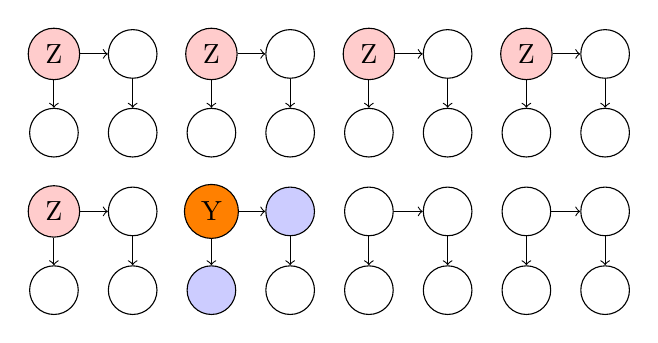
\begin{tikzpicture}[nodes={draw, circle}, ->]
        \node[fill = red!20] (3) at (0,1) {Z};
        \node (1) at (1,1) {\phantom{0}};
        \node (0) at (1,0) {\phantom{0}};
        \node (2) at (0,0) {\phantom{0}};
        \draw [->] (3) -- (1);
        \draw [->] (3) -- (2);
        \draw [->] (1) -- (0);
        \node[fill = red!20] (7) at (2,1) {Z};
        \node  (5) at (3,1) {\phantom{0}};
        \node (4) at (3,0) {\phantom{0}};
        \node (6) at (2,0) {\phantom{0}};
        \draw [->] (7) -- (5);
        \draw [->] (7) -- (6);
        \draw [->] (5) -- (4);
        \node[fill = red!20] (11) at (0,-1) {Z};
        \node (9) at (1,-1) {\phantom{0}};
        \node (8) at (1,-2) {\phantom{0}};
        \node (10) at (0,-2) {\phantom{0}};
        \draw [->] (11) -- (9);
        \draw [->] (11) -- (10);
        \draw [->] (9) -- (8);
        \node[fill = orange] (27) at (2,-1) {Y};
        \node[fill = blue!20]  (13) at (3,-1) {\phantom{0}};
        \node (12) at (3,-2) {\phantom{0}};
        \node[fill = blue!20]  (14) at (2,-2) {\phantom{0}};
        \draw [->] (27) -- (13);
        \draw [->] (27) -- (14);
        \draw [->] (13) -- (12);
        
        \node[fill = red!20] (11) at (4,1) {Z};
        \node (9) at (5,1) {\phantom{0}};
        \node (8) at (5,0) {\phantom{0}};
        \node (10) at (4,0) {\phantom{0}};
        \draw [->] (11) -- (9);
        \draw [->] (11) -- (10);
        \draw [->] (9) -- (8);
        \node[fill = red!20] (15) at (6,1) {Z};
        \node (13) at (7,1) {\phantom{0}};
        \node (12) at (7,0) {\phantom{0}};
        \node (14) at (6,0) {\phantom{0}};
        \draw [->] (15) -- (13);
        \draw [->] (15) -- (14);
        \draw [->] (13) -- (12);
        \node  (23) at (4,-1) {\phantom{0}};
        \node (9) at (5,-1) {\phantom{0}};
        \node (8) at (5,-2) {\phantom{0}};
        \node (26) at (4,-2) {\phantom{0}};
        \draw [->] (23) -- (9);
        \draw [->] (23) -- (26);
        \draw [->] (9) -- (8);
        \node  (19) at (6,-1) {\phantom{0}};
        \node (13) at (7,-1) {\phantom{0}};
        \node (12) at (7,-2) {\phantom{0}};
        \node (14) at (6,-2) {\phantom{0}};
        \draw [->] (19) -- (13);
        \draw [->] (19) -- (14);
        \draw [->] (13) -- (12);
\end{tikzpicture}}
\caption{\label{fig:fenwick_tree_cells_example_2} Hybrid mapping with $2\times 2$ cells showing the qubit operator representation of $\frac{i}{2}(a_{27}-a^{\dagger}_{27})$. Orange = target, Blue = Flip set, Red = Parity set}
\end{figure}
\begin{figure}[hbtp] 
        \centerline{
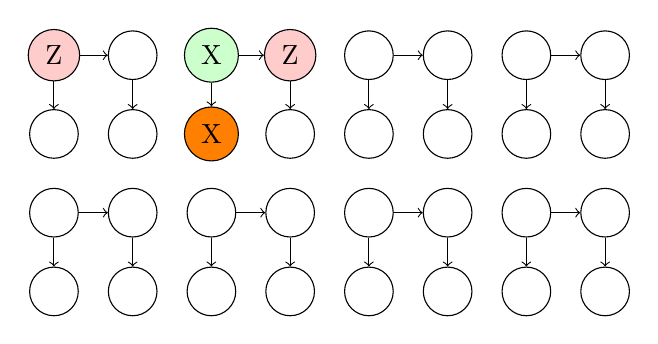
\begin{tikzpicture}[nodes={draw, circle}, ->]
        \node[fill = red!20] (3) at (0,1) {Z};
        \node (1) at (1,1) {\phantom{0}};
        \node (0) at (1,0) {\phantom{0}};
        \node (2) at (0,0) {\phantom{0}};
        \draw [->] (3) -- (1);
        \draw [->] (3) -- (2);
        \draw [->] (1) -- (0);
        \node[fill = green!20] (7) at (2,1) {X};
        \node[fill = red!20]  (5) at (3,1) {Z};
        \node (4) at (3,0) {\phantom{0}};
        \node[fill = orange] (6) at (2,0) {X};
        \draw [->] (7) -- (5);
        \draw [->] (7) -- (6);
        \draw [->] (5) -- (4);
        \node (11) at (0,-1) {\phantom{0}};
        \node (9) at (1,-1) {\phantom{0}};
        \node (8) at (1,-2) {\phantom{0}};
        \node (10) at (0,-2) {\phantom{0}};
        \draw [->] (11) -- (9);
        \draw [->] (11) -- (10);
        \draw [->] (9) -- (8);
        \node (27) at (2,-1) {\phantom{0}};
        \node  (13) at (3,-1) {\phantom{0}};
        \node (12) at (3,-2) {\phantom{0}};
        \node  (14) at (2,-2) {\phantom{0}};
        \draw [->] (27) -- (13);
        \draw [->] (27) -- (14);
        \draw [->] (13) -- (12);
        
        \node (11) at (4,1) {\phantom{0}};
        \node (9) at (5,1) {\phantom{0}};
        \node (8) at (5,0) {\phantom{0}};
        \node (10) at (4,0) {\phantom{0}};
        \draw [->] (11) -- (9);
        \draw [->] (11) -- (10);
        \draw [->] (9) -- (8);
        \node (15) at (6,1) {\phantom{0}};
        \node (13) at (7,1) {\phantom{0}};
        \node (12) at (7,0) {\phantom{0}};
        \node (14) at (6,0) {\phantom{0}};
        \draw [->] (15) -- (13);
        \draw [->] (15) -- (14);
        \draw [->] (13) -- (12);
        \node  (23) at (4,-1) {\phantom{0}};
        \node (9) at (5,-1) {\phantom{0}};
        \node (8) at (5,-2) {\phantom{0}};
        \node (26) at (4,-2) {\phantom{0}};
        \draw [->] (23) -- (9);
        \draw [->] (23) -- (26);
        \draw [->] (9) -- (8);
        \node  (19) at (6,-1) {\phantom{0}};
        \node (13) at (7,-1) {\phantom{0}};
        \node (12) at (7,-2) {\phantom{0}};
        \node (14) at (6,-2) {\phantom{0}};
        \draw [->] (19) -- (13);
        \draw [->] (19) -- (14);
        \draw [->] (13) -- (12);
\end{tikzpicture}}
\caption{\label{fig:fenwick_tree_cells_example_3} Hybrid mapping with $2\times 2$ cells showing the qubit operator representation of $\frac{1}{2}(a_{6}+a^{\dagger}_{6})$. Orange = target, Red = Parity set, Green = Update set}
\end{figure}
\begin{figure}[hbtp] 
        \centerline{
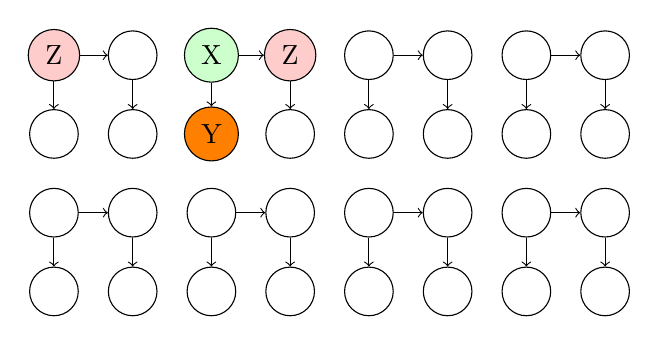
\begin{tikzpicture}[nodes={draw, circle}, ->]
        \node[fill = red!20] (3) at (0,1) {Z};
        \node (1) at (1,1) {\phantom{0}};
        \node (0) at (1,0) {\phantom{0}};
        \node (2) at (0,0) {\phantom{0}};
        \draw [->] (3) -- (1);
        \draw [->] (3) -- (2);
        \draw [->] (1) -- (0);
        \node[fill = green!20] (7) at (2,1) {X};
        \node[fill = red!20]  (5) at (3,1) {Z};
        \node (4) at (3,0) {\phantom{0}};
        \node[fill = orange] (6) at (2,0) {Y};
        \draw [->] (7) -- (5);
        \draw [->] (7) -- (6);
        \draw [->] (5) -- (4);
        \node (11) at (0,-1) {\phantom{0}};
        \node (9) at (1,-1) {\phantom{0}};
        \node (8) at (1,-2) {\phantom{0}};
        \node (10) at (0,-2) {\phantom{0}};
        \draw [->] (11) -- (9);
        \draw [->] (11) -- (10);
        \draw [->] (9) -- (8);
        \node (27) at (2,-1) {\phantom{0}};
        \node  (13) at (3,-1) {\phantom{0}};
        \node (12) at (3,-2) {\phantom{0}};
        \node  (14) at (2,-2) {\phantom{0}};
        \draw [->] (27) -- (13);
        \draw [->] (27) -- (14);
        \draw [->] (13) -- (12);
        
        \node (11) at (4,1) {\phantom{0}};
        \node (9) at (5,1) {\phantom{0}};
        \node (8) at (5,0) {\phantom{0}};
        \node (10) at (4,0) {\phantom{0}};
        \draw [->] (11) -- (9);
        \draw [->] (11) -- (10);
        \draw [->] (9) -- (8);
        \node (15) at (6,1) {\phantom{0}};
        \node (13) at (7,1) {\phantom{0}};
        \node (12) at (7,0) {\phantom{0}};
        \node (14) at (6,0) {\phantom{0}};
        \draw [->] (15) -- (13);
        \draw [->] (15) -- (14);
        \draw [->] (13) -- (12);
        \node  (23) at (4,-1) {\phantom{0}};
        \node (9) at (5,-1) {\phantom{0}};
        \node (8) at (5,-2) {\phantom{0}};
        \node (26) at (4,-2) {\phantom{0}};
        \draw [->] (23) -- (9);
        \draw [->] (23) -- (26);
        \draw [->] (9) -- (8);
        \node  (19) at (6,-1) {\phantom{0}};
        \node (13) at (7,-1) {\phantom{0}};
        \node (12) at (7,-2) {\phantom{0}};
        \node (14) at (6,-2) {\phantom{0}};
        \draw [->] (19) -- (13);
        \draw [->] (19) -- (14);
        \draw [->] (13) -- (12);
\end{tikzpicture}}
\caption{\label{fig:fenwick_tree_cells_example_4} Hybrid mapping with $2\times 2$ cells showing the qubit operator representation of $\frac{i}{2}(a_{6}-a^{\dagger}_{6})$. Orange = target, Red = Parity set, Green = Update set}
\end{figure}
It is important to note that while we have presented the Hybrid mapping in terms of the even fermionic operators (keeping inline with the Hybrid\+ mapping which can only represent even fermionic operators), it can also admit a representation of the whole fermionic space. \Cref{fig:fenwick_tree_cells,fig:fenwick_tree_cells_example_1,fig:fenwick_tree_cells_example_2,fig:fenwick_tree_cells_example_3,fig:fenwick_tree_cells_example_4} illustrate in detail how the odd fermionic operators are mapped, and it is clear how to construct the even fermionic operators by multiplying these together.
\subsubsection{Hybrid\+ mapping algorithm}
\label{section:auxHybridmapping}
\noindent
\textbf{Input:} \textit{$N\times N$ Fermion Square-Lattice Interaction Graph, Cell Shape $n \times n$}, $n \times n = 2^k$ for some integer $k$, $n$ is a factor of $N$\\
\textbf{Output:} \textit{Pauli-strings corresponding to interaction edges, Enumerated square-lattice of qubits plus required ancillas, Preprocessing entanglement gates}\\
\textbf{Summary:} This algorithm essentially extends the Jordan-Wigner portion of the Hybrid mapping scheme in the same way AQM extends the Jordan-Wigner mapping. We add in an ancilla per tree and then perform entangling operators upon the roots of the trees and the ancillas such that particular stabiliser operations are constructed. We can then use these stabilisers to shorten non-local strings on the roots of the trees to a single operation on an ancilla.\\
\textbf{Algorithm:}
\begin{enumerate}
    \item Perform steps 1-4 of the Hybrid mapping algorithm, but alternatively assign the \textit{cell number} ($c_i$) in a S pattern (illustrated by Figure~\ref{SPattern} in Appendix~\ref{appendix}).
    \item For every cell $c_i$, add one ancilla to the qubit enumeration scheme. This ancilla qubit is labelled $(c_i, n \times n +1)$ and only needs to be connected to the root of the cell $(c_i, n\times n)$ and the ancillas of the neighbouring cells.
    \item Prepare a stabiliser for each ancilla containing the string of Z gates involved in performing a fermionic operation between the roots of the current cell and the cell vertically above.
    (A detailed description of these stabilisers is given in Appendix~\ref{appendix} Figure~\ref{fig:stabilisers}). The stabilisers are created using the method described in \cite{steudtner2019quantum} by applying the following series of entangling gates: 
    \begin{enumerate}
        \item Apply a Hadamard gate to every ancilla 
        \item Entangle the edges of the rows by applying either of the gates controlled by the ancilla C shown in Figure~\ref{fig:entangleEdge} depending on the direction of the S-pattern on the row.
        \begin{figure}
          \centering
        \includegraphics[page=4, width=0.5\textwidth  , height=6cm]{Hybrid_Fermion_Mapping_diagrams.pdf}
        \caption{\label{fig:entangleEdge}Gates performed on edges of rows conditional upon the ancillas at the end of each row labeled with $C$.  The dashed boxes represent the cells, whilst the circles inside them represent the roots of each cell, and the circles without boxes represent the ancillas.}
    \end{figure}
    \item Move along each row applying either of the gates controlled by ancilla C shown in Figure~\ref{fig:entangleRow} depending on the direction of the S-pattern on the row.
   \begin{figure}
    \centering
        \includegraphics[page=5, width=0.5\textwidth  , height=6cm]{Hybrid_Fermion_Mapping_diagrams.pdf}
        \caption{\label{fig:entangleRow}Examples from the two (for odd/even rows) series of gates applied conditional upon the ancillas labeled with $C$. Each element in the series is identical to the previous but shifted one row to the left (odd rows) or right (even rows). The first element in each series is the 2nd rightmost (odd rows) and 2nd leftmost (even rows).}
    \end{figure}
    \\\\This technique exploits the newly created stabiliser of the previously entangled ancilla to cancel out most of the gates required to entangle the next ancilla in the row.
    \end{enumerate}
    \item For each interaction edge in your fermion interaction graph between $(c_1, f_1)$ and $(c_2, f_2)$ generate the Pauli-string representation:
    \begin{enumerate}
        \item Perform steps 5a)-c) of the Hybrid mapping algorithm
        \item We will only consider physical (even) fermionic operations, i.e. those which preserve the fermion number parity. For example:
        \begin{dmath*}
                    a_1a^{\dagger}_2 +a_2a^{\dagger}_1  \rightarrow X_{U_1}  \sigma^-_1  Z_{P_1/F_1}  X_{U_2}  \sigma^+_2Z_{P_2/F_2} +  X_{U_2}  \sigma^-_2  Z_{P_2/F_2}  X_{U_1}  \sigma^+_1Z_{P_1/F_1}
                    \rightarrow \frac{1}{2}\bigotimes_{j \in (U_1 \oplus U_2)} X_j \bigotimes_{k \in (P_1/F_1 \oplus P_2/F_2)} Z_k \> \\ \left( X_{(c_1, f_1)} \otimes X_{(c_2, f_2)} \bigotimes_{k \in F_1} Z_k \bigotimes_{j \in F_2} Z_j  + Y_{(c_1, f_1)}  \otimes Y_{(c_2, f_2)} \right) 
            \end{dmath*}
        In what follows we only need to consider how these operators act on the roots of the cells $(c_i, n\times n)$, as the stabiliser only deals with the cell roots. As $n\times n = 2^k$ each cell will contain a connected Fenwick tree, so each root will either be in the update set or be one of the targets. Therefore, each root is either acted on by $X_{(c_i, f_i)} $ or $X_{(c_t, f_t)} \otimes X_{(c_i, f_i)} \bigotimes_{k \in F_t} Z_k \bigotimes_{j \in F_i} Z_j  + Y_{(c_t, f_t)}  \otimes Y_{(c_i, f_i)} $. 
        \item We need to modify every string so they preserve the stabilisers. For each stabiliser, add a Z gate (acting on the associated ancilla) to every string that anti-commutes with the stabiliser. We are also able to shorten long S pattern Pauli strings by multiplying by appropriate stabilisers. Figure~\ref{fig:verticalInteractionXodd} demonstrates how the Hybrid\+ mapping modifies a Pauli-string representing a local fermionic operation in the Hybrid mapping scheme. Further examples are illustrated by Figures~\ref{fig:verticalInteractionYodd} and \ref{fig:horizontalInteractionXYYX} in Appendix~\ref{appendix}.\\\\
        If neither of the target fermions are the roots of their cell then the fermionic operation (on the level of cell roots) will simply be $XZ \ldots ZX$. However, if one of them is a root it will also include terms such as $XZ\ldots ZY$ and $YZ \ldots ZX$ (and potentially $YZ\ldots ZY$ if they are both roots).
        % We have used the same stabilisers described in https://arxiv.org/pdf/1810.02681.pdf
        % Describing them is difficult as they vary depending on the line, also uses S ordering rather than Z ordering so does not match with the previous mapping here
   \begin{figure}[hbpt]
    \centering
        \includegraphics[page=6, width=0.5\textwidth , height=6cm]{Hybrid_Fermion_Mapping_diagrams.pdf}\\
        \tikz[baseline=-\baselineskip]\draw[ultra thick,->] (0,0) -- ++ (0,-1);\\
        \includegraphics[page=7, width=0.5\textwidth , height=6cm]{Hybrid_Fermion_Mapping_diagrams.pdf}\\
        \tikz[baseline=-\baselineskip]\draw[ultra thick,->] (0,0) -- ++ (0,-1);\\
        \includegraphics[page=8, width=0.5\textwidth  , height=6cm]{Hybrid_Fermion_Mapping_diagrams.pdf}
        \caption{\label{fig:verticalInteractionXodd}Diagram showing how the Pauli-string representing a vertical hopping term (top) is modified by the Hybrid\+ mapping algorithm. First, Z gates are added to all the ancillas with associated stabilisers that anti-commute with the string (middle). Then, a stabiliser shown in Figure~\ref{fig:stabilisers} is applied canceling out a large portion of the string to give the final local operation (bottom)}
    \end{figure}
    \end{enumerate}
\end{enumerate}
\subsection{Algorithm analysis}
\label{section:algorithmanalysis}
% Graphs showing performance of our two algorithms
% Theoretical explanation of speed up offered by Hybrid
\subsubsection{Theoretical Average Pauli-weight of $n\times n$ Hybrid on an $N\times N$ lattice}
\label{section:hybridanalysis}
There are two primary contributions to the Pauli-weight of a fermionic operation in the Hybrid scheme:
\begin{enumerate}
    \item Local (Bravyi-Kitaev type) gates acting on qubits within the target cells
    \item Non-local (Jordan-Wigner type) gates acting on the roots of the cells between the two target cells in the Z-pattern
\end{enumerate}
The first contribution scales with $O(\log(n^2))$, whereas the second contribution scales with $O(N)$.

We can analytically calculate the second contribution:
\begin{itemize}
    \item Any interactions within a single cell make no contributions here
    \item Horizontal interaction terms between cells only contribute the root of one the target cells. However, as this root will already either be the target or in the update set we can ignore this contribution.
    \item Vertical interaction terms between qubits in different cells contribute $\frac{N}{n} -1$. Therefore, the total contributions from each row is:
    \begin{equation}
            \sum_{i=1}^{N} \frac{N}{n} -1 = N\left(\frac{N}{n} -1\right)
    \end{equation}
    Therefore, as there are $\frac{N}{n}$ rows the total of the second contribution is:
    \begin{equation}
        \frac{N^2}{n}\left(\frac{N}{n}-1\right)
    \end{equation}
    As there are $2N(N - 1)$ interactions in the whole lattice this gives the following contribution to the average Pauli-weight:
    \begin{equation}
        \frac{N}{2(N-1)n}\left(\frac{N}{n}-1\right)
    \end{equation}
\end{itemize}
Therefore, the average Pauli-weight of $n\times n$ Hybrid on an $N\times N$ lattice is:
\begin{equation}
        \frac{N(N-n)}{2(N-1)n^2} + O(\log n) 
\end{equation}
and so for large lattices:
\begin{equation}
        \frac{N}{2n^2} + O(\log n) 
\end{equation}
When $N\gg n$, the Hybrid mapping produces $n^2$ times smaller Pauli-strings than the Jordan-Wigner mapping.
% Theoretical constant performance of Hybrid\+ mapping
\subsubsection{Theoretical Average Pauli-weight of $n\times n$ Hybrid\+ on an $N\times N$ lattice}
Similarly to the Hybrid mapping, there are two primary contributions to the Pauli-weight of a fermionic operation:
\begin{enumerate}
    \item Local (Bravyi-Kitaev type) gates acting on qubits within the target cells
    \item Local (AQM type) gates acting on ancilla qubits
\end{enumerate}
The first contribution scales with $O(\log(n^2))$, whereas the second contribution scales with $O(\frac{1}{n})$ (as the ratio of inter-cell/intra-cell interactions decreases as $n$ increases). Therefore, as $N$ (and therefore the number of fermionic modes) increases the average Pauli-weight will remain constant.

\subsubsection{Varying impact of connectivity}
\label{section:connectivity}
The limitations of the underlying qubit architecture has a large impact on the performance of various mappings. In this section, we demonstrate the advantages our mappings give over existing schemes when used on a quantum computer with the common square-lattice connectivity. The connectivity constraints impact mappings by requiring SWAP gates to perform entangled operations between physically non-local qubits. In our analysis, we compare the number of qubits acted upon by a Pauli or SWAP gate during a fermionic operation (the \textit{range}). Below we consider the varying impact of connectivity upon different mappings.

\textbf {Jordan-Wigner Mapping}. The Jordan-Wigner mapping only requires a linear connectivity mapping, so it requires no additional gates to use on a square-lattice of qubits. However, it has been shown that an optimal choice of enumeration can give a constant improvement in the Pauli weight~\cite{chiew2021optimal}.

% Explanation of how Bravyi-Kitaev is reduced in performance to level of Jordan-Wigner when considering SWAP gates
\textbf {Bravyi-Kitaev Mapping}.
The Bravyi-Kitaev mapping requires a very high level of connectivity. In order to avoid any additional gates one must be able to embed an $\log N$ degree graph (the Fenwick tree) within the qubit architecture. As a square-lattice of connectivity has degree $4$ it is not possible to embed a Bravyi-Kitaev mapping of more than 16 fermionic modes. Therefore, for Bravyi-Kitaev mappings on larger systems neighbouring Fenwick tree nodes will not be connected, so additional SWAP gates are required to perform entangled gates on these qubits.

We found that simulating these additional SWAP gates drastically reduced the performance of the Bravyi-Kitaev mapping. This is theoretically supported by considering the scaling of the largest range interactions. Consider the fermionic operation between the fermions corresponding to qubits which are physically located at opposite ends of a row (or column), this operation must include these qubits as they are the targets. To connect just these two qubits at least $N$ qubits must be involved in the operation. Our unoptimized Z-pattern enumeration for the Bravyi-Kitaev mapping includes non-local interactions such as these, and hence the average range scales with $O(N)$. It is feasible that an optimal Bravyi-Kitaev enumeration could be found that scales more favourably. However, this is a very hard problem as the number of possible enumeration schemes grows factorially with lattice size and there is no known solution.

\textbf {Hybrid mapping}.
The main strength of this mapping is its performance in the real-world scenario of a square-lattice connectivity. It combines the Jordan-Wigner mappings connectivity flexibility with the Bravyi-Kitaev mappings increased locality. The average interaction qubit count contribution from within the Bravyi-Kitaev cells scales as above with $O(n)$. While the Pauli operations on the roots of the cells along the S-pattern are joined up with SWAP gates making the contribution per row from vertical interactions:
\begin{equation}
        \sum_{i=1}^{N} (N-1) = N(N-1)
\end{equation}
Therefore, as there are $\frac{N}{n}$ rows and $2N(N-1)$ interactions in the whole lattice, the contribution to the average range is:
\begin{equation}
     \frac{N}{2n}
\end{equation}
Therefore, the average range scales with $O(n + \frac{N}{2n})$. So for $N \gg n$, this mapping has $n$ times lower average range than both the Bravyi-Kitaev and Jordan-Wigner mappings.

\textbf {Hybrid\+ mapping}.
This algorithm requires a slightly higher level of connectivity. Our formulation has a second square-lattice of ancilla qubits connected to the original at the roots of the cells. It could also be formulated by instead choosing one qubit in each cell of the original square lattice to be an ancilla. However, we chose our formulation as it produces a lower range, is simpler to consider, and still is a realistic qubit architecture.

The Hybrid\+ mapping retains a constant average Pauli-weight when considering the limitations of connectivity. This is due to the only rising contribution coming from the Bravyi-Kitaev mapping within the target cells which should scale with roughly $O(n)$, and for a given mapping $n$ is constant.
\begin{figure}[hbpt]
    \centering
    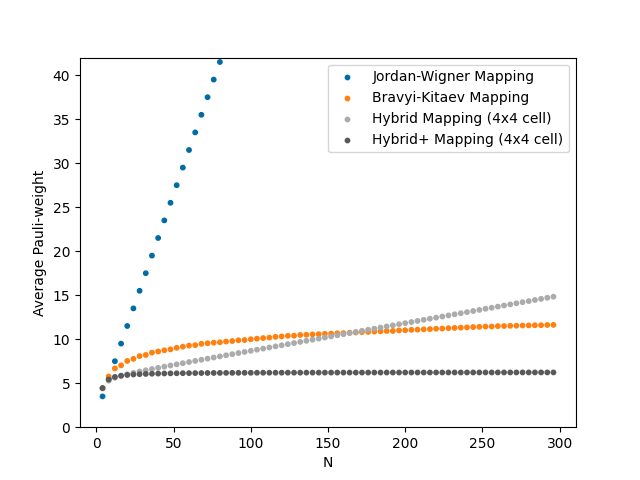
\includegraphics[width = 0.5\textwidth]{compare_mappings_average_qubit_nums_ex_SWAP.png}
    \caption{The average Pauli-weight of fermionic operations on an $N\times N$ lattice against $N$ when using a given mapping.}
    \label{fig:compare_mappings_ex_SWAP}
\end{figure}
\begin{figure}[hbpt]
    \centering
    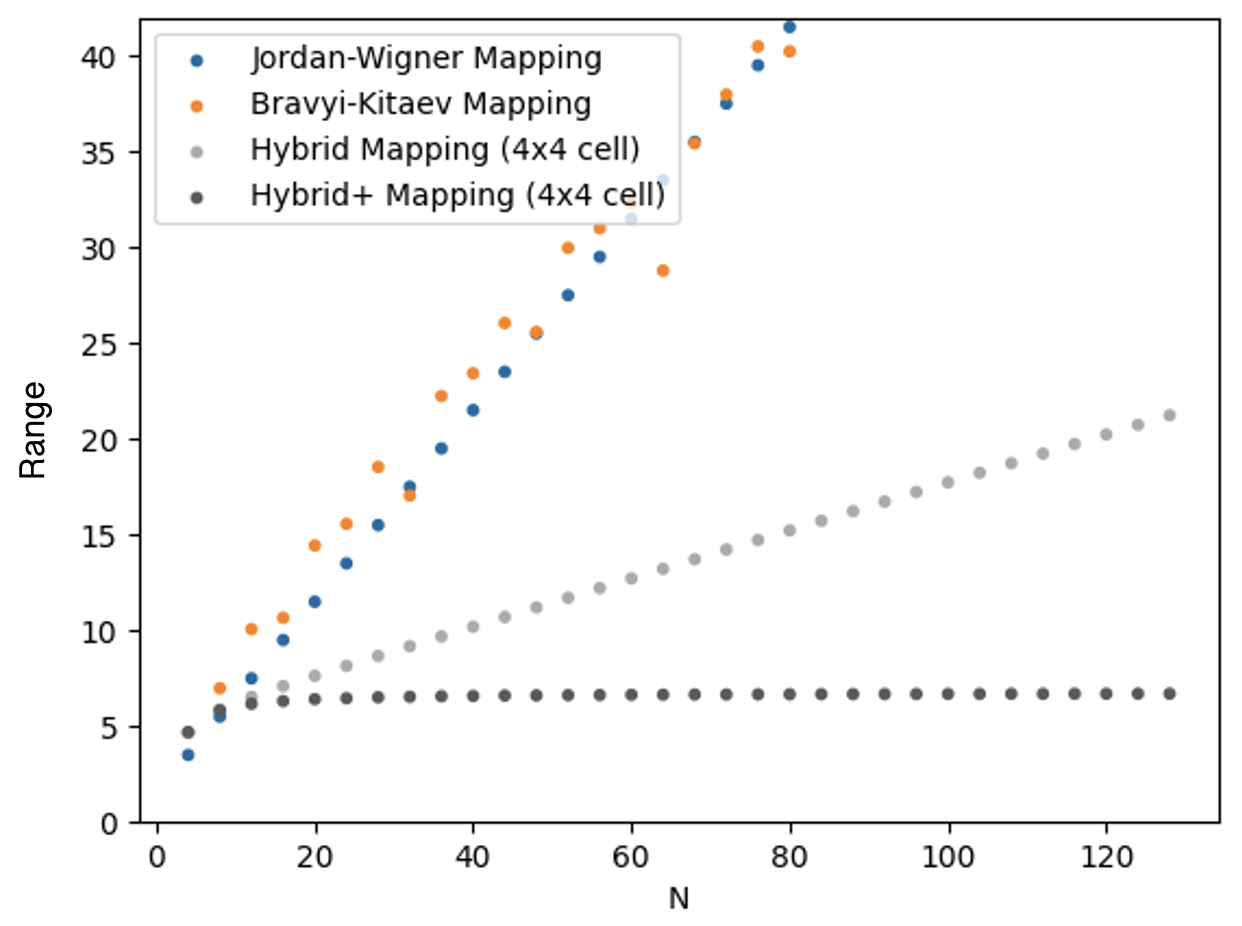
\includegraphics[width = 0.5\textwidth]{compare_mappings_average_qubit_nums.TMP.png}
     \caption{The average range of each fermionic operation on an $N\times N$ lattice against $N$ when using a given mapping in the context of a square-lattice qubit connectivity.}
    \label{fig:compare_mappings}
\end{figure}
\begin{figure}[hbpt]
    \centering
    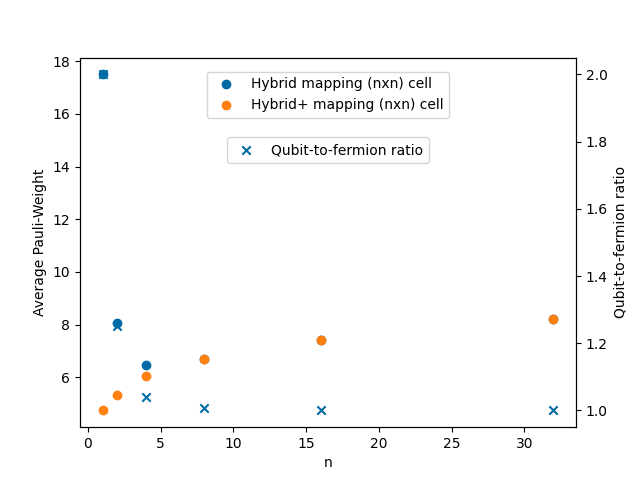
\includegraphics[width = 0.5\textwidth]{vary_cell_sizes_average_qubit_nums_ex_SWAP_03_11_2022.png}
    \caption{The average Pauli-weight of a fermionic operation on an $32\times 32$ lattice when using an $n\times n$ Hybrid/Hybrid\+ mapping against $n$. The crosses denote the qubit-to-fermion ratio of the $n\times n$ Hybrid\+ mapping for each choice of $n$.}
    \label{fig:vary_cell_sizes_ex_SWAP}
\end{figure}
\begin{figure}[hbpt]
    \centering
    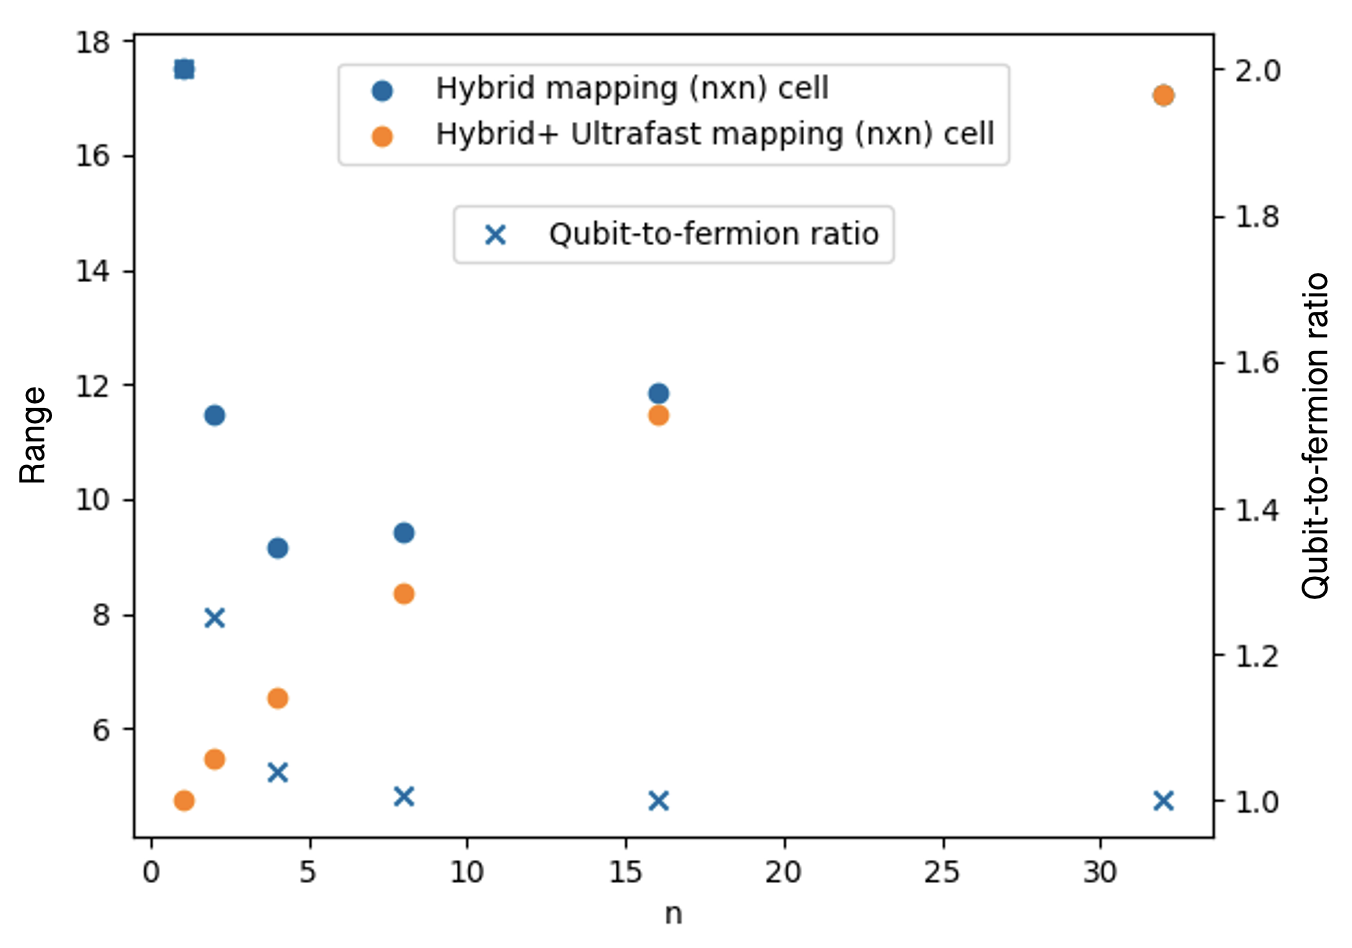
\includegraphics[width = 0.5\textwidth]{vary_cell_sizes_average_qubit_nums_03_11_2022.png}
    \caption{The average range of each fermionic operation on an $32\times 32$ lattice when using an $n\times n$ Hybrid/Hybrid\+  mapping against $n$ in the context of a square-lattice qubit connectivity.The crosses denote the qubit-to-fermion ratio of the $n\times n$ Hybrid\+ mapping for each choice of $n$.}
    \label{fig:vary_cell_sizes_32}
\end{figure}
\begin{figure}[hbpt]
    \centering
    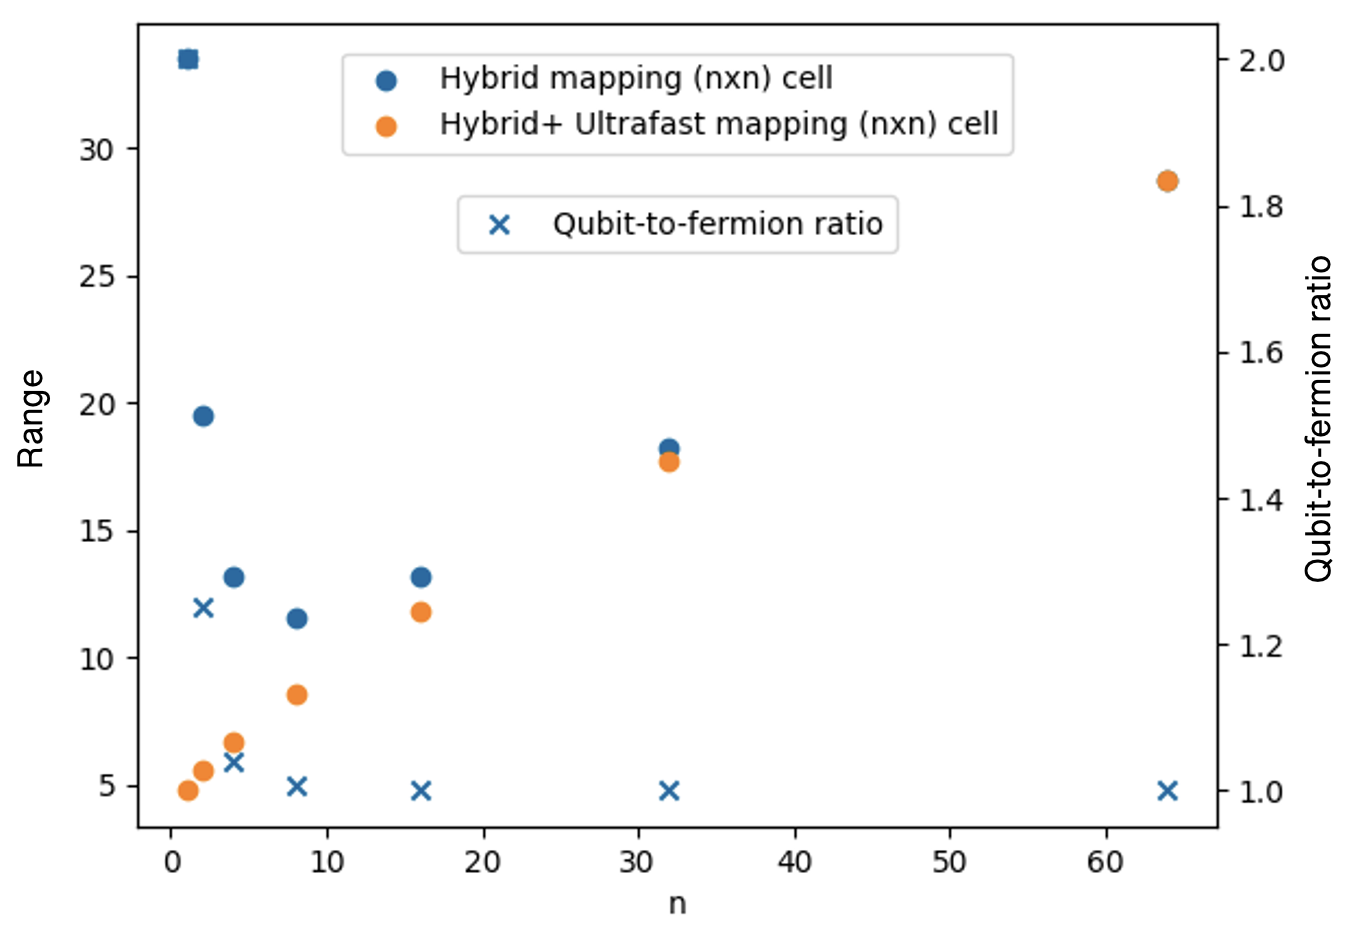
\includegraphics[width = 0.5\textwidth]{vary_cell_sizes_average_qubit_nums_07_11_2022.png}
    \caption{The average range of each fermionic operation on an $64\times 64$ lattice when using an $n\times n$ Hybrid/Hybrid\+  mapping against $n$ in the context of a square-lattice qubit connectivity for $n=\{1,2,4,8,16,32,64\}$. These results include qubits solely acted on by SWAP gates. The crosses denote the qubit-to-fermion ratio of the $n\times n$ Hybrid\+ mapping for each choice of $n$.}
    \label{fig:vary_cell_sizes_64}
\end{figure}
\begin{figure}[hbpt]
    \centering
    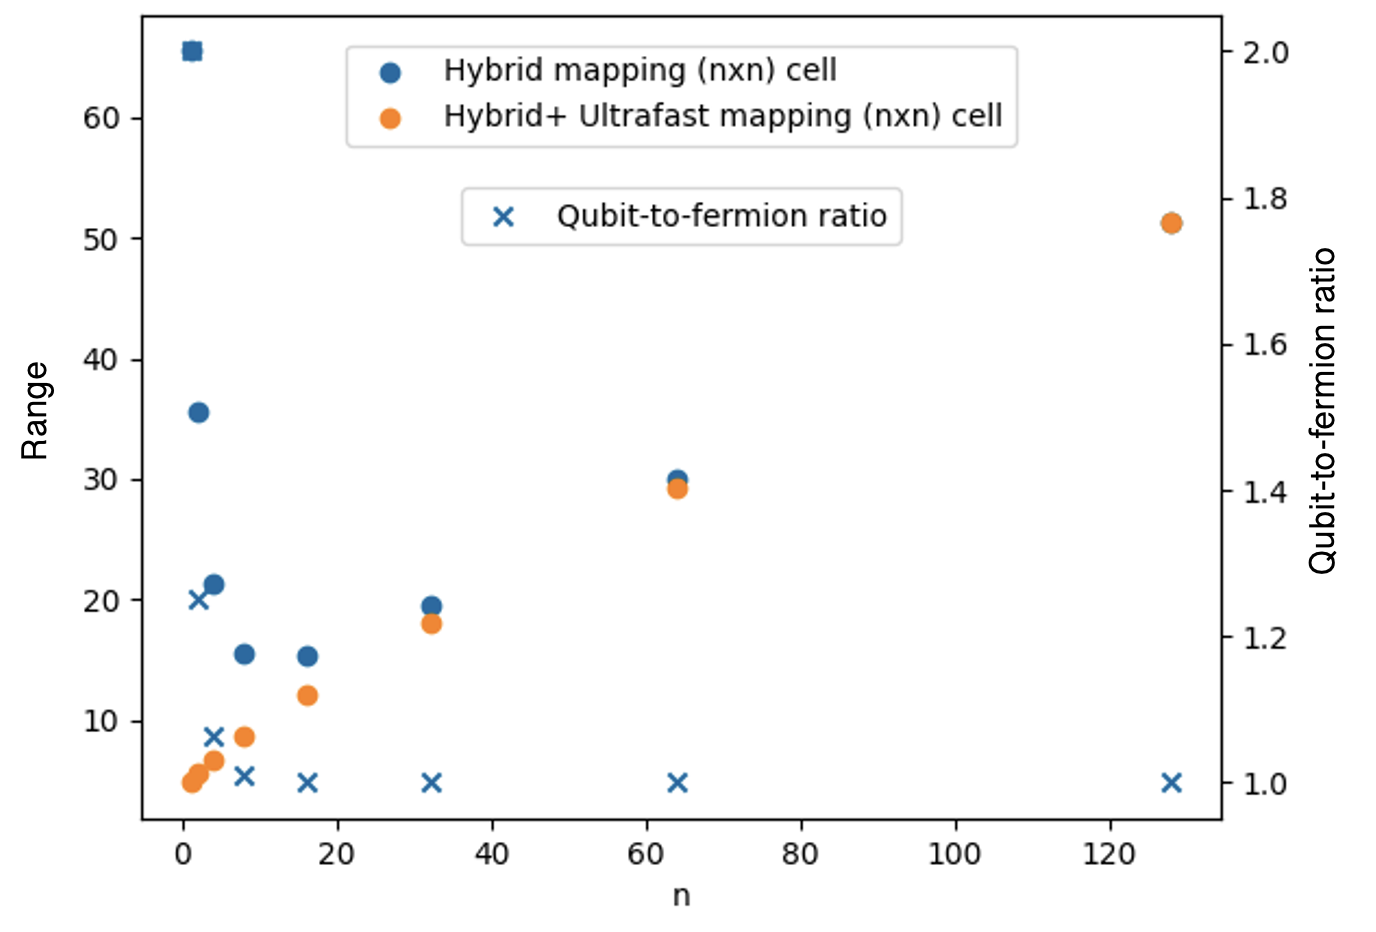
\includegraphics[width = 0.5\textwidth]{vary_cell_sizes_average_qubit_nums.128.TMP.png}
    \caption{The average range of each fermionic operation on an $128\times 128$ lattice when using an $n\times n$ Hybrid/Hybrid\+  mapping against $n$ in the context of a square-lattice qubit connectivity for $n=\{1,2,4,8,16,32,64,128\}$. These results include qubits solely acted on by SWAP gates. The crosses denote the qubit-to-fermion ratio of the $n\times n$ Hybrid\+ mapping for each choice of $n$.}
    \label{fig:vary_cell_sizes_128}
\end{figure}
\subsubsection{Numerical Analysis}
\label{section:numerical}
We have considered the locality of each algorithm by computing the average range on a $N \times N$ square lattice. When investigating the case of a $4 \times 4$ cell, we found that the theoretical predictions held; the average interaction qubit count scaled with $\frac{N}{32}$ for the Hybrid algorithm and asymptotically approached a constant for the Hybrid\+ algorithm (as illustrated in Figure~\ref{fig:compare_mappings_ex_SWAP}).

We performed the same analysis in the context of an underlying square lattice connectivity. This required calculating the minimum number of SWAP gates required to connect all the qubits involved in the operation. We approximated the solution to this Steiner Tree problem using the SCIP-JACK library outlined in Appendix~\ref{section:SCIPJACK}. Figure~\ref{fig:compare_mappings} shows that the theoretical predictions hold with the average range increasing with $\frac{N}{8}$ for the Hybrid algorithm and tending to a constant for the Hybrid\+ algorithm.

The largest difference evident is in the Bravyi-Kitaev mapping. When including SWAP gates, the average range involved appears to be scaling linearly rather than logarithmically. In our calculations we used a trivial Z-pattern enumeration scheme for the Bravyi-Kitaev mapping, so it is possible the performance could be improved by an optimal choice of enumeration scheme.

Therefore in the context of an underlying square lattice connectivity the $4 \times 4$ Hybrid mapping out-performs both the Jordan-Wigner and Bravyi-Kitaev mapping by a factor of $4$ . Furthermore, even with all-to-all connectivity it still outperforms the Jordan-Wigner mapping by a factor of $16$, and beats the Bravyi-Kitaev mapping for lattices smaller than $164 \times 164$.

We have investigated which cell sizes give optimal performance. The behaviour shown in Figure~\ref{fig:vary_cell_sizes_ex_SWAP} and ~\ref{fig:vary_cell_sizes_32} matches with our theoretical predictions. For the Hybrid mapping, in the regime of $n \ll N$ the average range scales with $O(\frac{1}{2n^2})$ (for fixed $N$). However, this is quickly dominated by the $O(\log n)$ growth of the Bravyi-Kitaev mapping within each cell. Therefore, as the logarithm dominates for $K\frac{N}{2n^2} < \log n$ (for constant $K$), we hypothesis that the optimal choice of $n$ will scale with roughly $O(\sqrt{N})$. The trend of increasing optimal choice of $n$ with lattice size is demonstrated by the increasing optimal cell size from $4\times 4$ to $8\times 8$ to $16 \times 16$ when the lattice size is increased from $32 \times 32$ (Figure~\ref{fig:vary_cell_sizes_32}) to $64 \times 64$ (Figure~\ref{fig:vary_cell_sizes_64}) to $128 \times 128$ (Figure~\ref{fig:vary_cell_sizes_128}).

For the Hybrid\+ mapping, there is no $O(\frac{1}{2n^2})$ regime as there are no non-local gates acting on the roots. Therefore, the behaviour is dominated by the Bravyi-Kitaev mapping within the cell. This is reflected in the $O(\log n)$ growth of average range. However, the optimal cell size is not simply the smallest (equivalent to AQM \cite{steudtner2019quantum}). The main benefit of this mapping is in offering a direct trade-off between number of ancillas and range. As the current minimum qubit-to-fermion ratio achieved by a local mapping is 1.25 \cite{chen2022equivalence}, we have analysed the next possible cell size of $4 \times 4$ which achieves a qubit-to-fermion ratio of 1.0625. However, using larger cell sizes requires far fewer ancilla qubits. For example, an $8 \times 8$ Hybrid\+ mapping requires 94\% fewer ancillas than the super-compact mapping scheme \cite{chen2022equivalence}.

\subsection{Discussion}
We have presented two novel mappings: the Hybrid mapping achieves the shortest circuits of all known mappings without ancillas. The margin of improvement is significant. As demonstrated in our simulations of a real-world qubit architecture, it generates $75\%$ lower range interactions than the Jordan-Wigner and Bravyi-Kitaev mappings. Additionally, as the lattice sizes increases the optimum cell size grows and the performance of the Hybrid mapping further improves.

For calculations on current or near-term quantum computers the Hybrid mapping demonstrates an improvement over the Bravyi-Kitaev and Jordan-Wigner mappings even with all-to-all connectivity. This holds for lattices up to $164 \times 164$ (Figure~\ref{fig:compare_mappings_ex_SWAP}). Lattices larger than this would require more than 27000 qubits to simulate, which is much larger than the current largest quantum computer (433 qubits~\cite{gambetta2020ibm}). Therefore, the Hybrid mapping will likely outperform the Bravyi-Kitaev and Jordan-Wigner mappings on real devices for the foreseeable future.

The Hybrid\+ mapping demonstrates a remarkable improvement on all existing local mapping schemes. It achieves similar levels of locality to the Derby-Klassen \cite{derby2021compact}, Super-compact \cite{chen2022equivalence}, and  AQM \cite{steudtner2019quantum} type mappings but expends only a small fraction of the ancillas in comparison. Our example of a $4 \times 4$ Hybrid\+ mapping required 75\% less ancillas than the local (super-compact) mapping with the lowest known ancilla requirements.

The Hybrid\+ mapping also provides a direct and simple trade-off between locality and ancilla qubits. Increasing the cell size $n$ increases the range linearly whilst the number of ancillas required decreases with $O(\frac{1}{n^2})$.

The approach we have taken in constructing both of these mappings need not be restricted to square-lattice qubit architectures. It should be possible to reproduce similar mappings for any architecture and corresponding fermionic interaction graph that admit a cellular decomposition.

We have considered a fermionic interaction graph which coincides with our architecture. It would be interesting to explore mapping an arbitrary fermionic interaction graph onto a given architecture using a similar Hybrid construct of connected Bravyi-Kitaev cells. In particular, we would like to understand how this mapping would translate into 3D, and whether this would require a 3D qubit connectivity or if cubic cells can be mapped to a planar grid efficiently.

In our analysis, we found connectivity constraints significantly hampered the Bravyi-Kitaev type terms in the mapping. Further work could explore this phenomenon in more detail. It is possible that an optimal choice of fermionic enumerations following the optimization techniques of~\cite{chiew2021optimal} could significantly reduce the impact of the connectivity constraints.

A lesser-known but equally remarkable role of fermion-to-qubit mappings is their role as duality transformations. The Jordan-Wigner transform~\cite{jordan1993paulische} can be regarded as an example of such a duality transform~\cite{henderson2022strong}. It maps spin Hamiltonians (such as XXZ chain) to simple fermionic systems which can be investigated by classical quantum chemistry techniques or by quantum means~\cite{nishimori2010elements,cao2019quantum}. Our two new families of fermion-to-qubit mappings could be interpreted as efficient duality transformations. Therefore, an interesting application of these hybrid mappings is the investigation of complex Hamiltonians.




